\documentclass[preview]{standalone}

\usepackage{amsmath}
\usepackage{amssymb}
\usepackage{stellar}

\hypersetup{
    colorlinks=true,
    linkcolor=black,
    urlcolor=blue,
    pdftitle={Stellar},
    pdfpagemode=FullScreen,
}

\begin{document}

\id{geofisica-tempi-geologici}
\genpage

\section{I tempi geologici}

\begin{snippet}{tempi-geologici-expl}
    \textbf{Importanza del fattore tempo:}
    il tempo è cruciale per comprendere molti fenomeni naturali. Ad esempio, l'erosione di una gola
    da parte di un fiume avviene su una scala temporale di centinaia, migliaia o milioni di anni.
    
    \textbf{Limitazioni delle misurazioni temporali umane:}
    \begin{itemize}
        \item Le misure temporali umane dirette vanno da frazioni di secondo a poche decine di anni;
        \item Alcuni fenomeni naturali, come movimenti delle masse d'aria e acqua e le variazioni
            climatiche stagionali, rientrano in questo intervallo di tempo.
    \end{itemize}
    
    \textbf{Durata di processi geologici:}
    molti processi geologici si estendono su scale temporali molto superiori alla vita umana.
    Ad esempio, la formazione di uno spessore di pochi decimetri di fango sul fondale marino può
    richiedere decine di migliaia di anni.
    
    \textbf{Geologia e tempo:}
    \begin{itemize}
        \item La geologia studia la storia della Terra, la composizione della crosta terrestre e i
            processi di formazione delle rocce;
        \item Per comprendere i fenomeni geologici, è essenziale considerare il fattore tempo.
    \end{itemize}
    
    \textbf{Età della Terra:}
    \begin{itemize}
        \item La Terra ha un'età stimata di 4.54 miliardi di anni;
        \item Questa vasta scala temporale è fondamentale per comprendere fenomeni geologici come
            l'erosione fluviale e il sollevamento di catene montuose.
    \end{itemize}
\end{snippet}

\begin{snippet}{geologic-clock-events-periods-it}
    \begin{figure*}[h]
        \begin{center}
            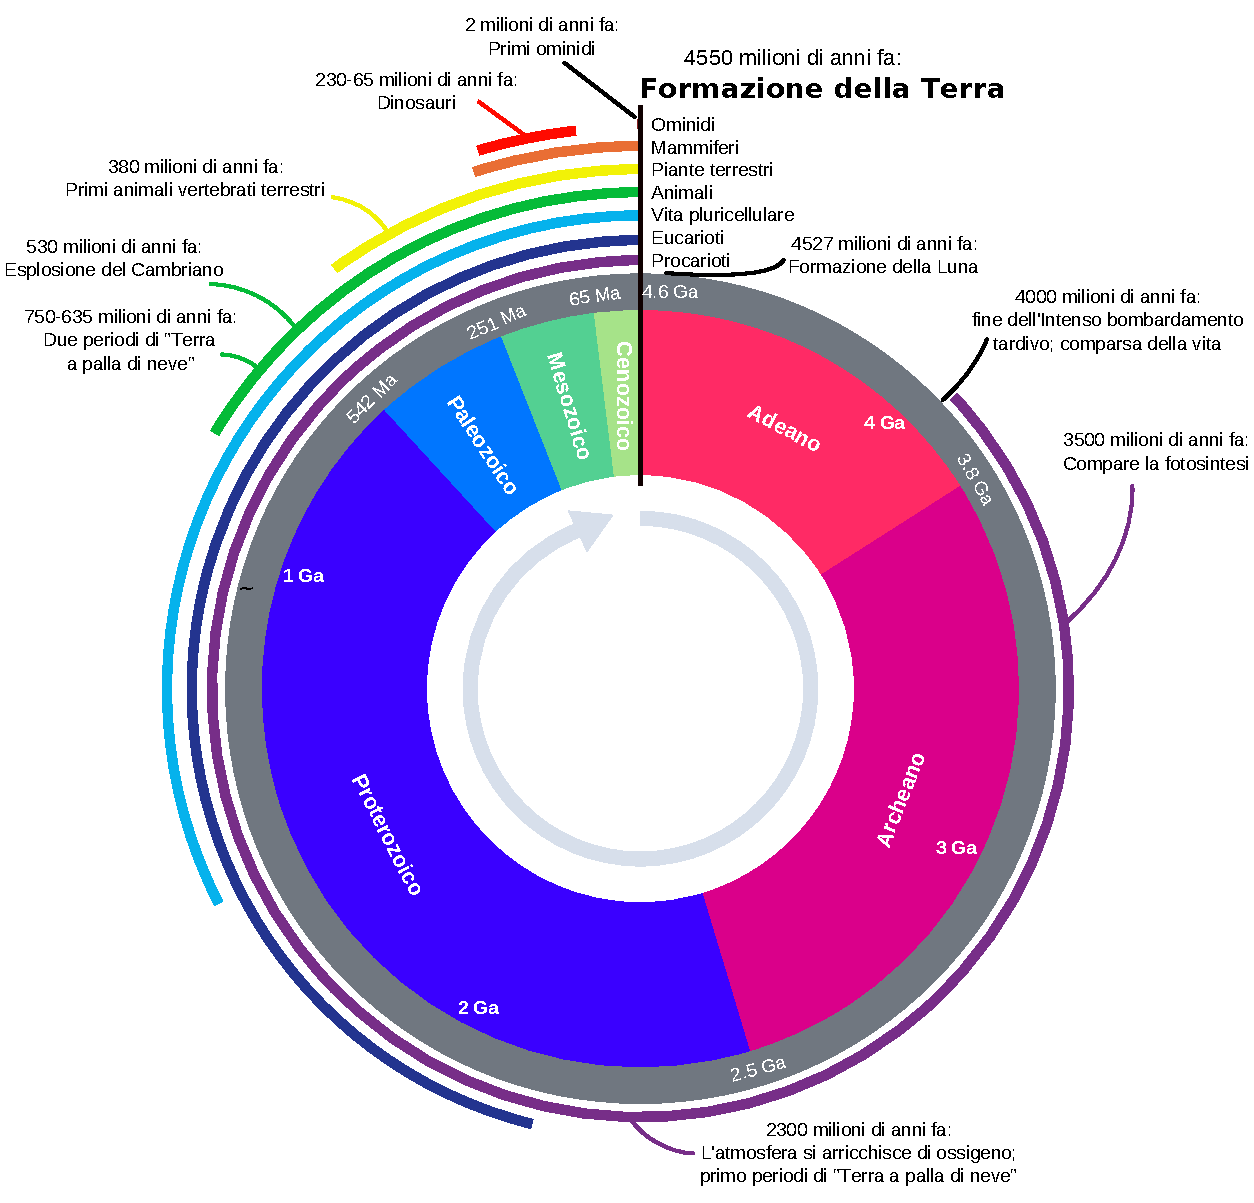
\includegraphics[width=.75\textwidth]{resources/geologic-clock-events-periods-it.pdf}
        \end{center}
    \end{figure*}
\end{snippet}

\end{document}